\label{chpt:results:three peculiar white dwarfs} % for referencing this chapter elsewhere, use \ref{chpt:label}
\lhead{\emph{Three CVs with peculiar white dwarf colours}} % This is for the header on each page - perhaps a shortened title


The work presented in this chapter was published as \cite{wild2021}, in the Monthly Notices of the Royal Astronomical Society under the title `\textit{System parameters of three short period cataclysmic variable stars}' by Wild, Littlefair, Ashley, Breedt, Brown, Dhillon, Dyer, Green, Kerry, Marsh, Parsons, and Sahman.
The following is my own work, unless otherwise cited.

This section concerns three systems, ASASSN-16kr, ASASSN-17jf, and CRTS SSSJ0522-3505 J052210-350530 (hereafter SSSJ0522-3505), which proved challenging to model.
The phase-folded eclipse modelling gave good results in all three systems, each lightcurve being well-modelled with small residuals -- for a catalogue of the fits, see Appendix~\ref{appendix:lightcurves}.
The Gaussian processes describing flickering in the systems were consistent with little to no variability, indicating that almost all the scatter in the flux residuals could be fully described by the uncertainty in flux measurement.
However, when fitting white dwarf model atmospheres to the observed white dwarf fluxes, the resulting fits were not satisfactory.


\begin{figure*}
    \centering
    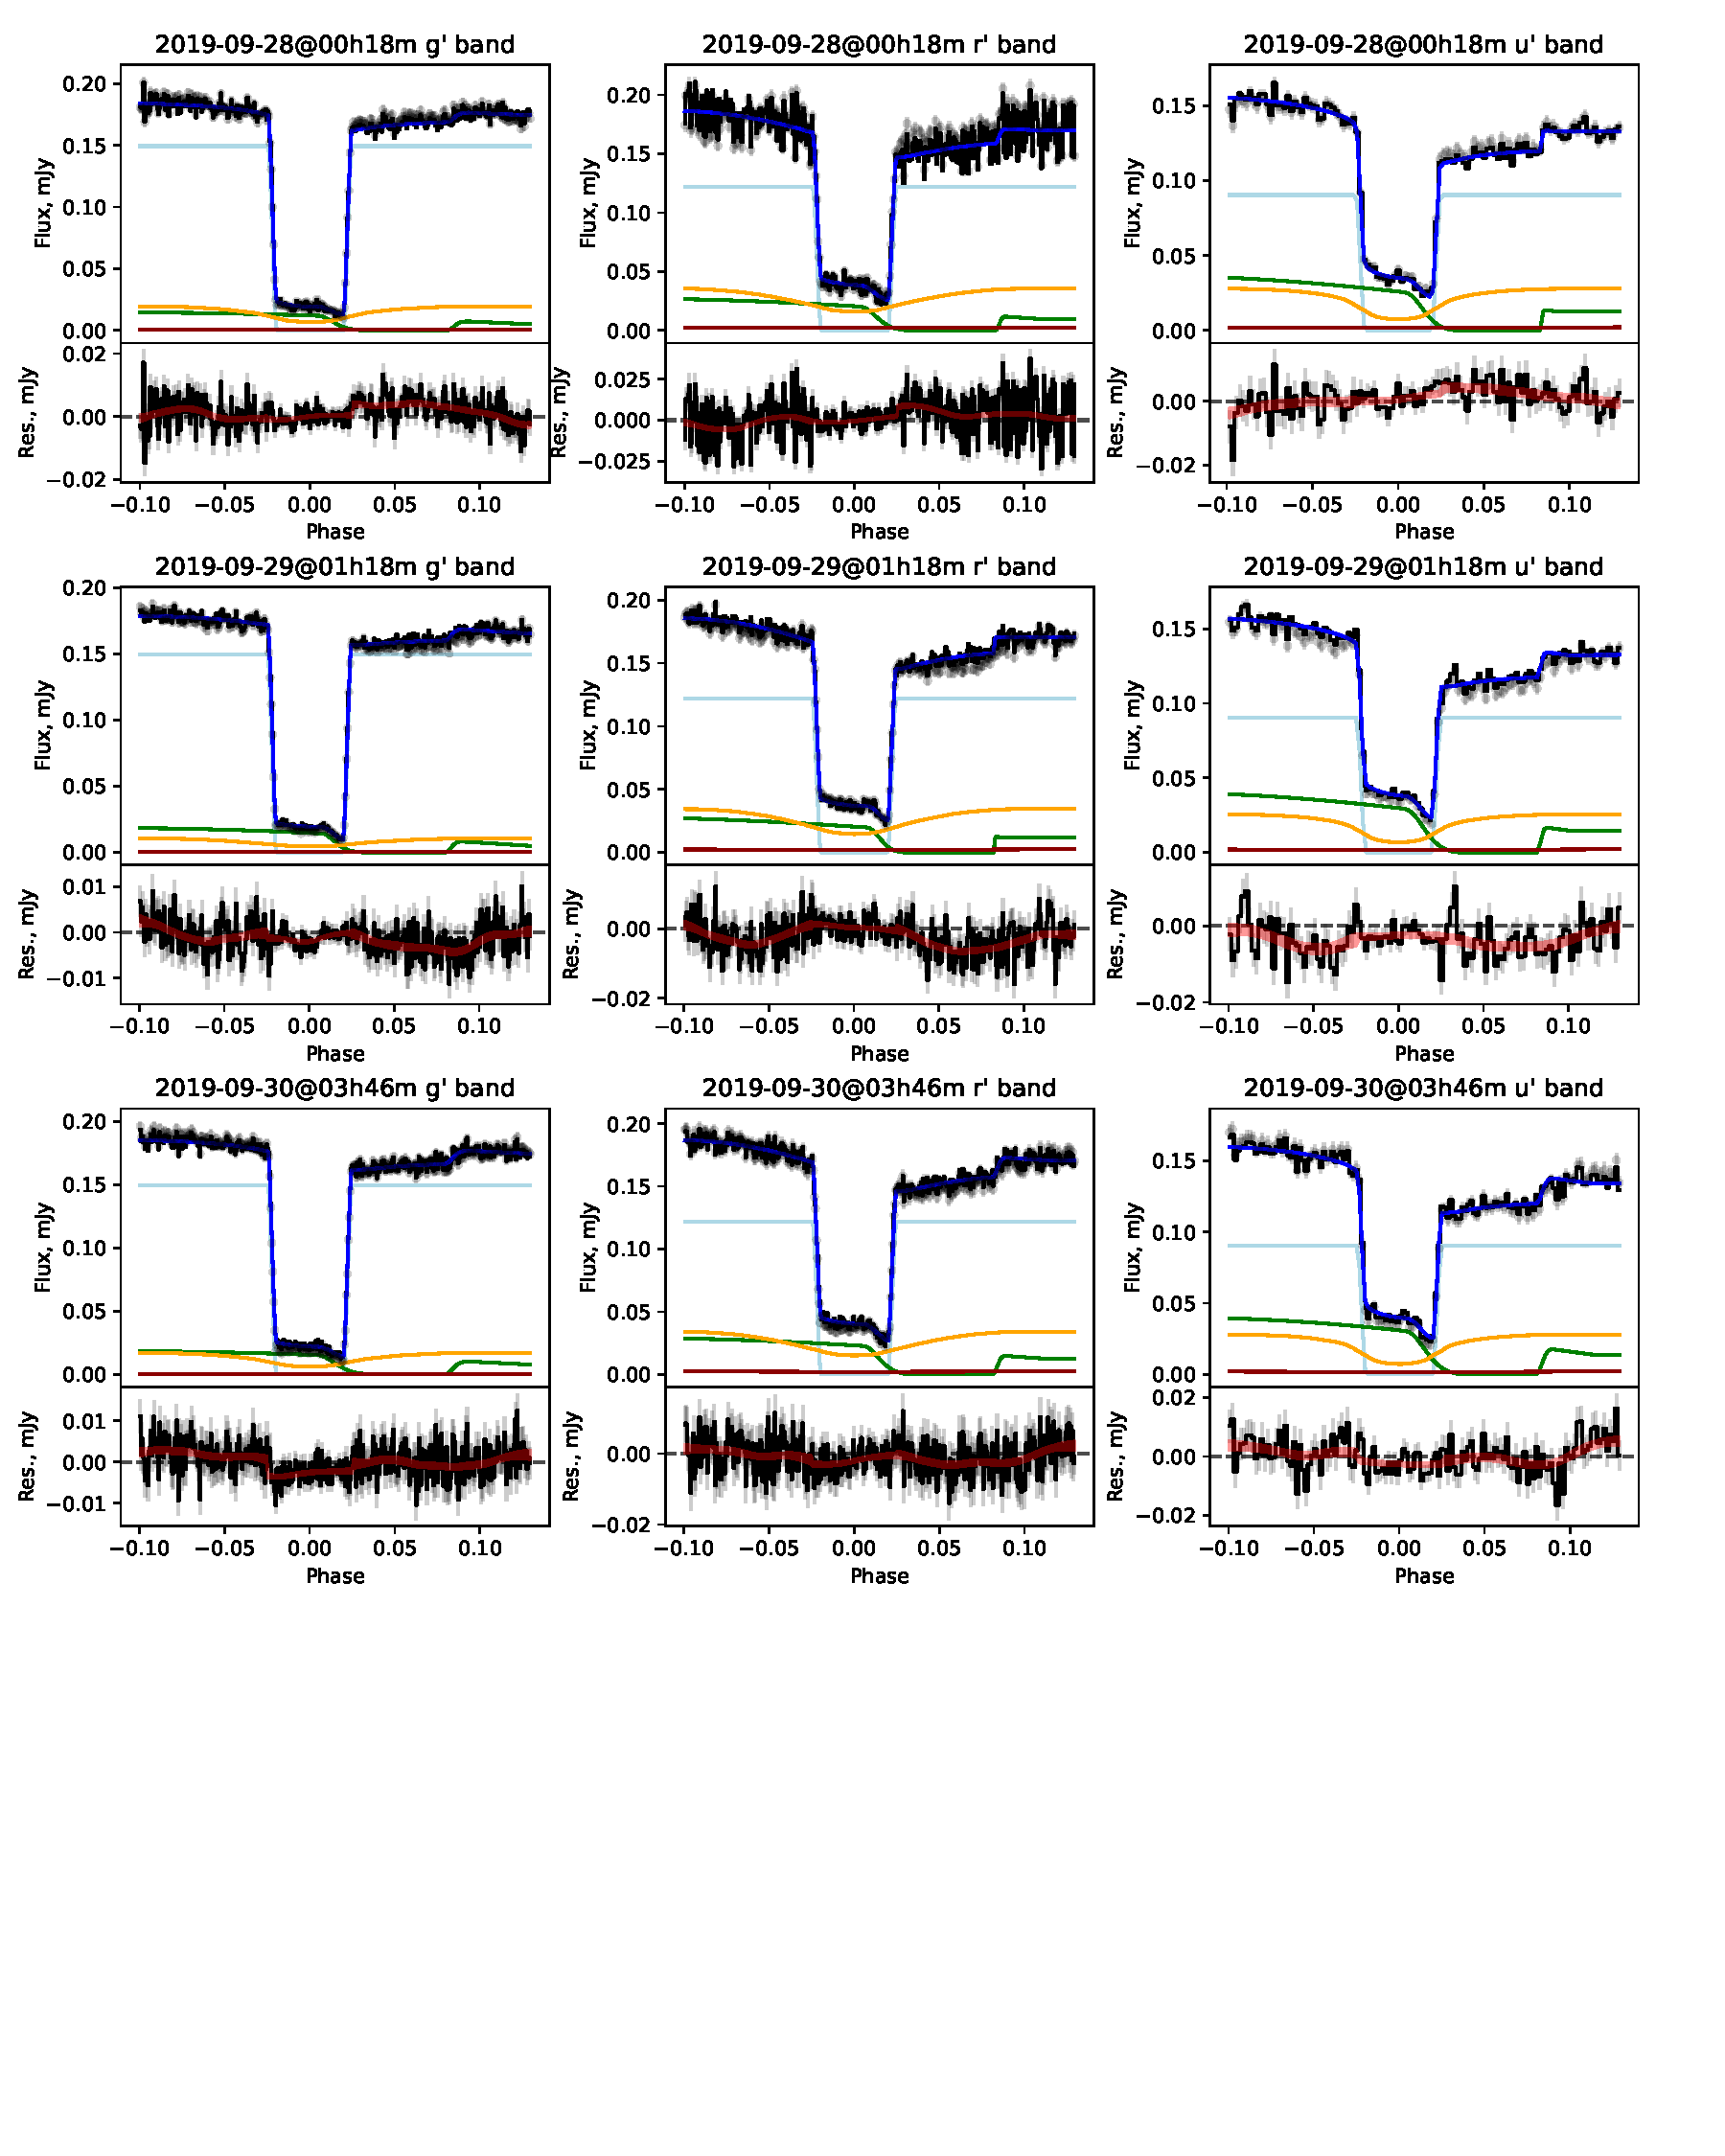
\includegraphics[width=\textwidth, trim={0.5 28.5cm 0.5 0}, clip]{figures/results/three_cvs_with_weird_colours/ASASSN-16kr/ASASSN-16kr_lightcurves_6.pdf}
    \caption{ASASSN-16kr example lightcurve models. {\it Top}:~grey points are the observed flux; black line is the observed flux, with the mean Gaussian process sample subtracted; the dark blue line is the mean lightcurve model, and the blue band is the standard deviation on this in the MCMC chain. The components of the model are also shown: the light blue line is the white dwarf flux, green line is the bright spot, orange line is the disc, and the red line is the donor. {\it Bottom}:~The residuals between the data and model are plotted as the black line, with grey error bars. The Gaussian process 1-sigma region is shown as a red band. A catalogue of all such fits in this work is given in Appendix~\ref{appendix:lightcurves}.}
    \label{fig:ASASSN-16kr example lightcurves}
\end{figure*}

\begin{table*}
    \centering
    \caption{The system parameters found for the three CVs with peculiar white dwarf colours.}
    \label{table:system_parameters}
    \begin{tabular}{cccc}
        \hline \\
        \textbf{System Name:}      & \textbf{ASASSN-16kr}    & \textbf{ASASSN-17jf}  & \textbf{SSSJ0522-3505} \\
        \hline \hline \\
        $M_\mathrm{WD}/M_\odot$    & $0.952\pm0.018$         & $0.669\pm0.031$        & $0.760\pm0.023$ \\
        $R_\mathrm{WD}/R_\odot$    & $0.0083\pm0.0002$       & $0.0120\pm0.0004$      & $0.0112\pm0.0003$ \\
        $M_\mathrm{donor}/M_\odot$ & $0.042\pm0.001$         & $0.060\pm0.008$        & $0.042\pm0.004$ \\
        $R_\mathrm{donor}/R_\odot$ & $0.105\pm0.002$         & $0.112\pm0.004$        & $0.105\pm0.004$ \\
        $q$                        & $0.044\pm0.002$         & $0.085\pm0.006$        & $0.055\pm0.003$ \\
        \hline
        $P$, hours            & $1.470862368 \pm 0.00000002$ & $1.36297 \pm 0.00002$  & $1.492642 \pm 0.0000002$ \\
        $a/R_\odot$,               & $0.653\pm0.005$         & $0.567\pm0.009$        & $0.614\pm0.007$  \\
        $i$\                       & $86.4\pm0.4$            & $83.7\pm0.5$           & $83.8\pm0.3$  \\
        $K_\mathrm{WD}$, km/s      & $22.7\pm1.5$            & $39.5\pm4.2$           & $26.0\pm1.8$  \\
        $K_\mathrm{donor}$, km/s   & $515\pm3$               & $462\pm5$              & $470\pm4$  \\
        \hline
        \plax, mas                 & $6.58\pm0.22$           & $2.09\pm0.19$          & $1.81\pm0.11$  \\
        \teff, kK                  & $10-12$                 & $8-13$                 & $\sim25$  \\
        ${\rm log}(g), {\rm cgs}$  & $8.55\pm0.03$           & $8.15\pm0.05$          & $8.22\pm0.04$  \\
        \hline
    \end{tabular}
\end{table*}


\subsection{White dwarf atmosphere fits}
\label{sect:method WD atmosphere fits}

The two values of log($g$) produced by modelling -- the first from fitting the white dwarf fluxes to model atmospheres, and the second from combining \teff\ and $P$\ with the lightcurve parameters -- did not fall within $1\sigma$\ of each other in any of these three systems.
In ASASSN-17jf and SSSJ0522-3505, the white dwarf atmosphere fit converged close to the minimum surface gravity allowed by the coverage of our models, ${\rm log}(g) = 7.0$.
The second log($g$), from lightcurve fitting, indicated values for each system of $8.10\pm0.04$ and $8.30\pm0.03$, respectively.
When analysing ASASSN-16kr, flux fitting gave a more reasonable ${\rm log}(g)=8.21\pm0.13$, but the second log($g$)\ still gave a significantly higher ${\rm log}(g)=8.59\pm0.03$, a difference of $\sim3\sigma$.

This is concerning, as the two log($g$)\ should be consistent with one another for each system.
Comparison of our measured white dwarf colours to the \citet{Bergeron1995} model grids in Figures \ref{fig:ASASSN-17jf colours}, \ref{fig:ASASSN-16kr colours}, and \ref{fig:SSSJ0522-3505 colours}, reveals that the measured colours of the white dwarfs lie outside the colour space of the models. This is the origin of the discrepancies in log($g$)\ obtained with the two methods for ASASSN-17jf and SSSJ0522-3505, but ASASSN-16kr appears consistent with the leftmost cooling track. However, the observed flux of a white dwarf of this radius is too high for the observed Gaia parallax, pushing the model fits to smaller, higher gravity model atmospheres.

A possible cause for this issue would be an error in photometric calibration, causing a corresponding error in white dwarf fluxes. However, this is unlikely to be the source of the problem, for the reasons explained in \S\ref{sec:observations:flux calibrating the lightcurve}.
Inspection of the figures in Appendix~\ref{appendix:lightcurves} also rules out poor lightcurve fits as the cause of this problem. The most plausible explanation for the fact that our measured white dwarf fluxes do not lie inside the model grids, is that the change in brightness during white dwarf ingress/egress is contaminated by an additional source of light, for example a boundary layer close to the white dwarf surface. The implications of this for our system parameters is discussed in \S\todo{add this in too}.

That the white dwarf colours do not lie on the model grids also raises questions about the accuracy of the white dwarf temperatures. To try and quantify the impact on \teff\, two additional optimisations of model parameters to the white dwarf fluxes were performed.
In one approach, a Gaussian prior on log($g$)\ using the estimate from the lightcurve modelling was used, and all available flux measurements.
In a second approach we fit the white dwarf flux in each band independently using the same prior on log($g$)\ and the Gaia prior on \plax. Since these independent fits use no colour information, E(B-V) is only constrained by the prior, but we retain it as a nuisance parameter and marginalise our \teff\ estimate over E(B-V). Figure~\ref{fig:gamma fits} shows the \teff\ posteriors from the individual fits for the three systems.

\begin{figure}
    \centering
    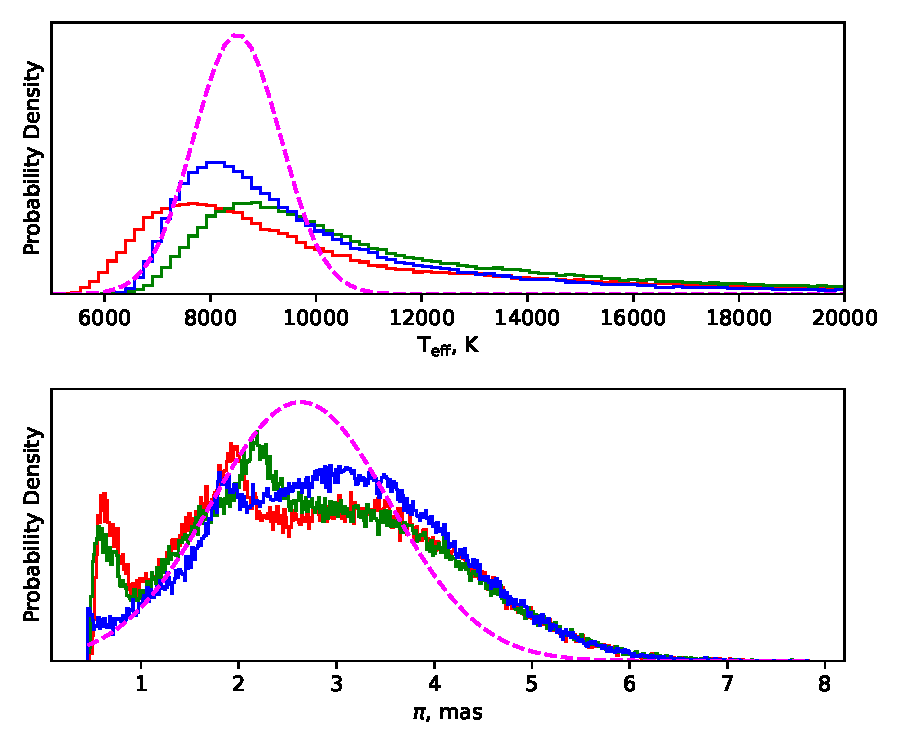
\includegraphics[width=\columnwidth, trim={0cm 6.5cm 0cm 0cm}, clip]{figures/results/three_cvs_with_weird_colours/ASASSN-17jf/PhysicalParams/all_gamma_asassn17jf.pdf}
    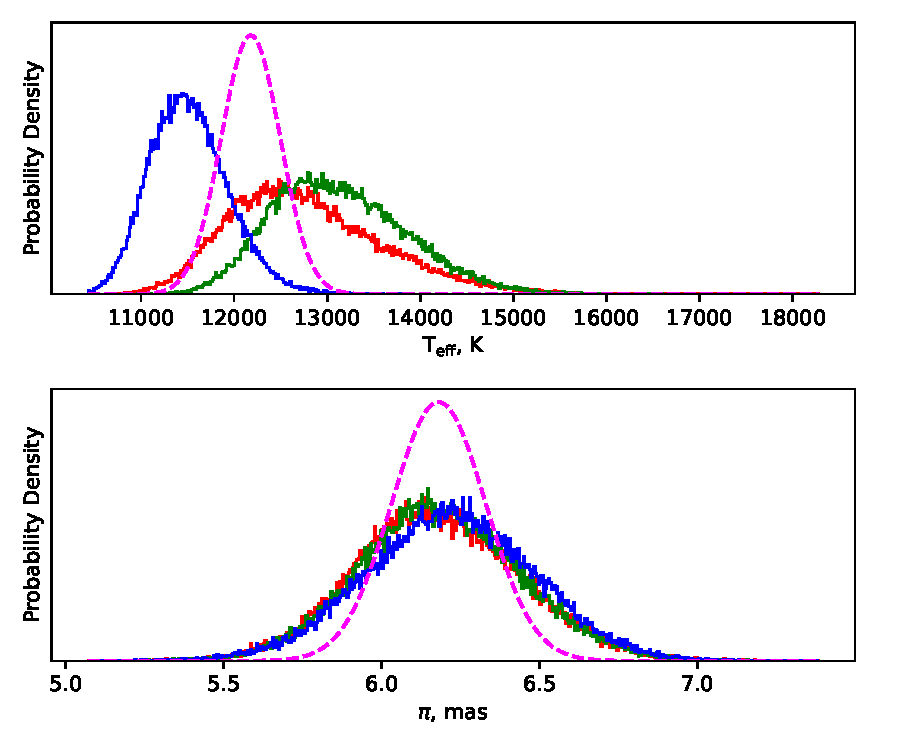
\includegraphics[width=\columnwidth, trim={0cm 6.5cm 0cm 0cm}, clip]{figures/results/three_cvs_with_weird_colours/ASASSN-16kr/PhysicalParams/all_gamma_asassn16kr.pdf}
    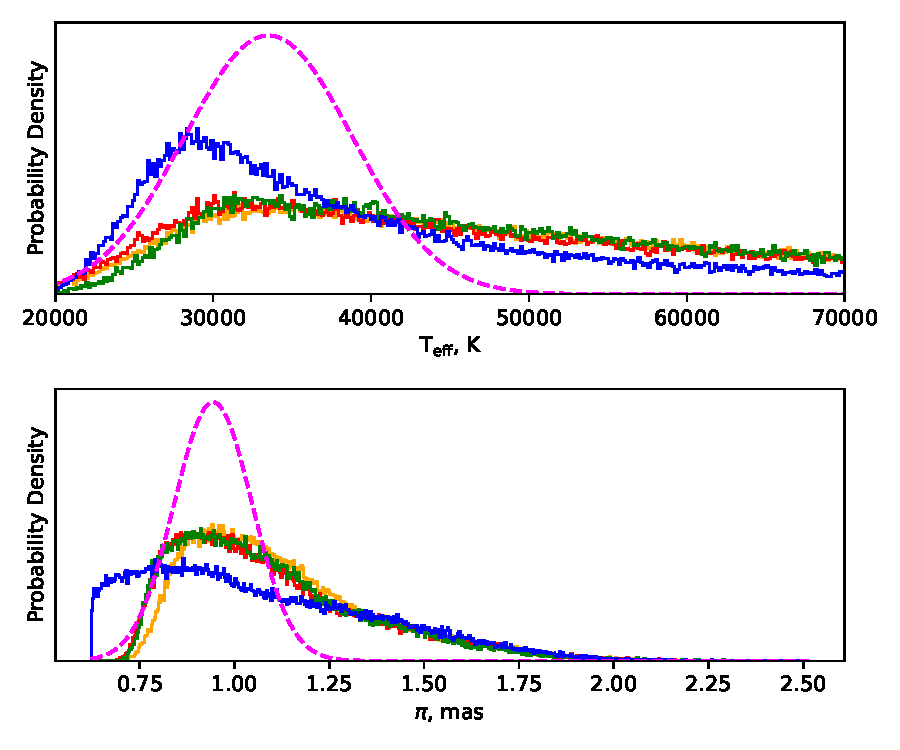
\includegraphics[width=\columnwidth, trim={0cm 6.5cm 0cm 0cm}, clip]{figures/results/three_cvs_with_weird_colours/SSS111126/PhysicalParams/all_gamma_SSS111126.pdf}
    \caption{The result of fitting white dwarf model atmospheres to each photometric band independently. Blue solid line: $u'$ band, Green solid line: $g'$ band, Red solid line: $r'$ band. The joint distribution between all bands is characterised in each case by the best fit Gaussian (magenta dashed lines). \textit{Top}: ASASSN-17jf, joint \teff$=8330\pm780\rm\ K$; \textit{Middle}: ASASSN-16kr, joint \teff$=12150\pm300\rm\ K$; \textit{Bottom}: SSSJ0522-3505, joint \teff$=33300\pm5200 \rm\ K$. }
    \label{fig:gamma fits}
\end{figure}

From Figure \ref{fig:gamma fits}, we can see that there is little sign of a consistent discrepancy over the three observed CVs. The $u'$ band in ASASSN-16kr and SSSJ0522-3505 suggests a cooler temperature than the other bands, but lies in between the $r'$ and $g'$ in ASASSN-17jf.


\subsubsection{White dwarf temperature fits}
\label{sect:white dwarf temperature report}

Each approach gives a different distribution for \teff.
To avoid confusion, we do not report the results of each individual fit, but summarise the overall temperature ranges for each system.

ASASSN-16kr \teff\ estimates ranged from 10200K to 12150K, and ASASSN-17jf estimates from 8330K to  12710K.
The SSSJ0522-3505 fits that used all four observed fluxes both converged on $\sim22700$K, but the single-flux fits all resulted in wide posterior distributions covering $25000 - 90000$K, with very weak peaks in the $\sim30000 - 50000$K range, seen in Figure~\ref{fig:gamma fits}.

In all three systems, the figures we report in Table~\ref{table:system_parameters} are the \teff\ produced by the constrained log($g$)\ fit with all fluxes simultaneously.
The log($g$)\ reported are the values found from the lightcurve parameters.


\subsection{System Parameters}
\label{sect:system parameters}

We note that the effect of the uncertain white dwarf temperatures on the system parameters, such as $M_{\rm wd}$, is negligible. For example, increasing \teff\ for ASASSN-17jf from 8000K to 12000K only changes $M_{\rm WD}$ by $0.001M_\odot$, compared to our statistical uncertainty of $0.031 M_\odot$. Even a large uncertainty in \teff\ only has a minor impact on the system parameters; for example a change in the WD temp for SSSJ0522-3505 from $10000$K to $20000$K only changes $M_{\rm WD}$ by $0.02 M_\odot$, comparable with the measurement uncertainty. The system parameters are reported in Table~\ref{table:system_parameters}.

ASASSN-16kr has a recorded superhump period, and now also a robust $q$ measurement. It can therefore be used to calibrate the superhump period excess, $\epsilon$ vs. $q$ relationship, as done in \citet{McAllister2019}, though with a more extreme mass ratio system than was available to them. The system was not confidently classed as exhibiting stage B or C stage superhumps, so we look at the results for both stages. Assuming the CV was in stage B, we calculate $q_B = 0.059\pm0.007$; assuming stage C and using the relevant relation from \citet{McAllister2019}, we calculate $q_C = 0.068\pm0.012$. In both cases, the estimated $q_\mathrm{B,C}$ is $\sim 2 \sigma$ higher than the observed value of $q = 0.044\pm0.002$. While a $2 \sigma$ difference is not a highly significant discrepancy, this may be preliminary evidence that the $\epsilon - q$ relation may over estimate $q$ for CVs at short periods, which has been suspected for some time \citep{pearson2007, knigge11}.

\begin{figure}
    \centering
    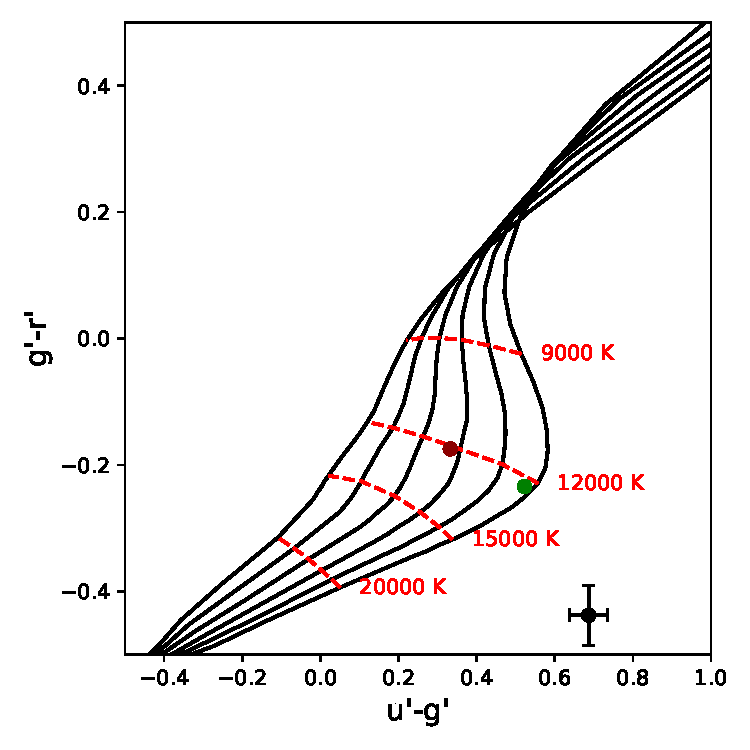
\includegraphics[width=\columnwidth, trim={0 0mm 0 0},clip]{figures/results/three_cvs_with_weird_colours/ASASSN-17jf/PhysicalParams/ASASSN-17jf_colourPlot_alpha_beta.pdf}
    \caption{The white dwarf model atmosphere fits for ASASSN-17jf. Green circle: Best fit with uniform prior on log($g$). Red circle: Best fit with the prior ${\rm log}(g)=8.10\pm0.04$. The observations are shown as the black point and error bars. Solid black lines are white dwarf model cooling tracks, increasing in log($g$)\ to the left. Red dashed lines are isothermal tracks for different log($g$).}
    \label{fig:ASASSN-17jf colours}
\end{figure}
\begin{figure}
    \centering
    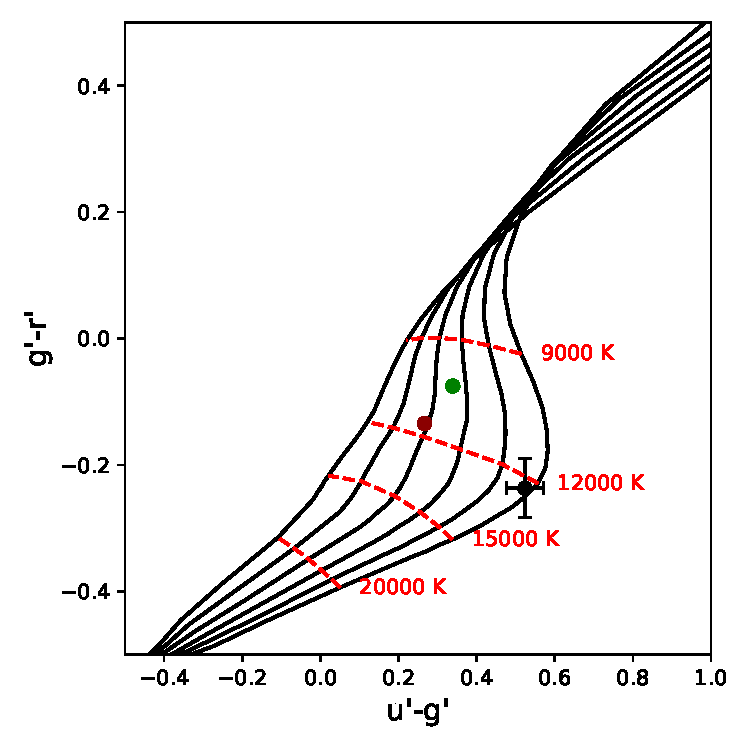
\includegraphics[width=\columnwidth, trim={0 0mm 0 0},clip]{figures/results/three_cvs_with_weird_colours/ASASSN-16kr/PhysicalParams/ASASSN-16kr_colourPlot_alpha_beta.pdf}
    \caption{The white dwarf model atmosphere fits for ASASSN-16kr. The red circle is the best fit with a prior of ${\rm log}(g)=8.52\pm0.02$. Symbols are the same as Figure~\ref{fig:ASASSN-17jf colours}.}
    \label{fig:ASASSN-16kr colours}
\end{figure}
\begin{figure}
    \centering
    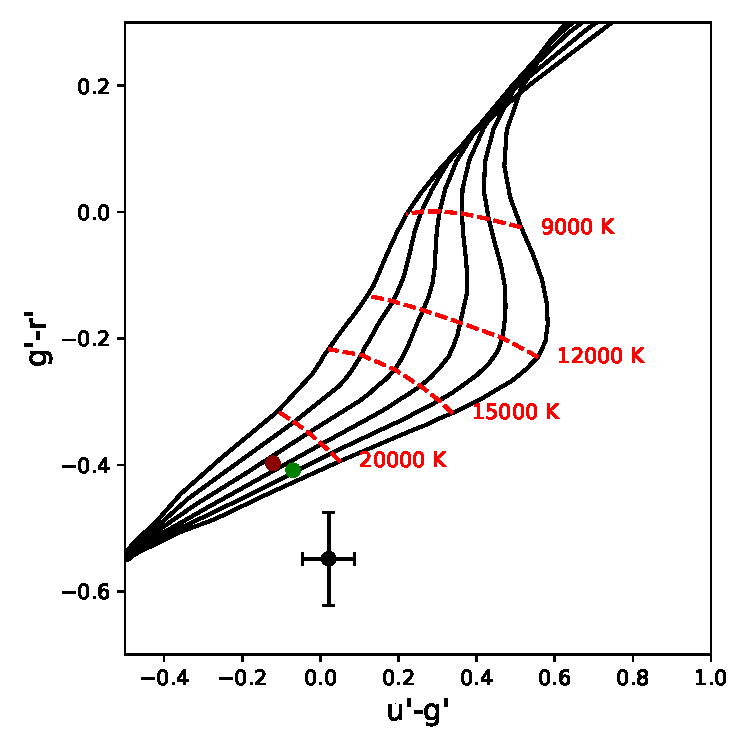
\includegraphics[width=\columnwidth, trim={0 0 0 0}, clip]{figures/results/three_cvs_with_weird_colours/SSS111126/PhysicalParams/SSS111126_colourPlot_alpha_beta.pdf}
    \caption{The white dwarf model atmosphere fits for SSSJ0522-3505. The red circle is the best fit with a prior of ${\rm log}(g)=8.28\pm0.04$. Symbols are the same as Figure~\ref{fig:ASASSN-17jf colours}.}
    \label{fig:SSSJ0522-3505 colours}
\end{figure}



\section{Evolutionary modelling of CVs with MESA}




